\documentclass[screen]{beamer}
\usepackage{listings}
\usepackage{color}
\usepackage{bold-extra}
\usepackage{wasysym}
\usepackage{beamerthemesplit}
\usepackage{graphicx}
\usepackage{tikz}
\usetheme{default}

\usepackage{underscore}
\usepackage{ifthen}
\usepackage{amsmath}
\usepackage{graphicx}
\usepackage{url}

\newcommand{\Tcg}{\textsc{Tcg}}
\newcommand{\code}[1]{\texttt{#1}}
\newcounter{premise}
\newcommand{\premise}[2]{
\ifthenelse{\equal{\arabic{premise}}{1}}{\\}{}%
    \setcounter{premise}{1}%
    #1\vdash#2%
}
\newcommand{\ifnotempty}[2]{\ifthenelse{\equal{#1}{}}{}{#2}}
\newcommand{\tcgrule}[5]{%
	\setcounter{premise}{0}%
$$%
    \ifnotempty{#1}{%
        \forall \left(#1\right)\;%
    }%
    \dfrac{%
	    \begin{array}[b]{l}%
	    #2%
            \end{array}%
    }{%
            #3%
    }%
    \;\ifnotempty{#4}{(\mathtt{#4}\ifnotempty{#5}{[\mathbf{#5}]})}%
$$%
}

\title{A Generator for Type Checkers}
\subtitle{A report on the PhD thesis by H. Gast (2004)}
\author{Andrey Breslav}
\institute{ITMO University, St. Petersburg / University of Tartu}


\begin{document}

\frame{\titlepage}

\begin{frame}[t,fragile]
%%%%%%%%%%%%%%%%%%%%%%%%%%%%%%%%%%%%%%%%%%%%%%%%%%%%%%%%%%%%%%%%%%%%%%%%%%%%%%%%%%%%%%%%%%%%%%%%%%%%%%%%%%%%%%
\frametitle{A workflow of a compiler}%
program -> lexer -> parser -> AST -> type checker -> YES | NO
%%%%%%%%%%%%%%%%%%%%%%%%%%%%%%%%%%%%%%%%%%%%%%%%%%%%%%%%%%%%%%%%%%%%%%%%%%%%%%%%%%%%%%%%%%%%%%%%%%%%%%%%%%%%%%
\end{frame}

\frame{
	\frametitle{Problem statement}

	Describe type checkers with a declarative language.\\
	Some features to support:
	\begin{itemize}
		\item Simply-typed $\lambda$-calculus
		\item Polymorphic \textbf{let}
		\item Mutually recursive functions
		\item Inheritance of classes in OOP
		\item Generic programming
		\item \ldots
	\end{itemize}
}

\begin{frame}[t,fragile]
%%%%%%%%%%%%%%%%%%%%%%%%%%%%%%%%%%%%%%%%%%%%%%%%%%%%%%%%%%%%%%%%%%%%%%%%%%%%%%%%%%%%%%%%%%%%%%%%%%%%%%%%%%%%%%
\frametitle{Workflow of \Tcg{}}%

\begin{figure}[htp]
\centering
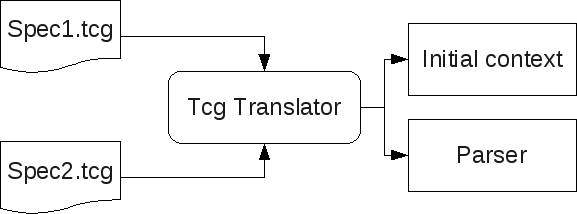
\includegraphics[width=.7\textwidth]{../generator}
\caption{The \Tcg{} Generator}
\end{figure}

%%%%%%%%%%%%%%%%%%%%%%%%%%%%%%%%%%%%%%%%%%%%%%%%%%%%%%%%%%%%%%%%%%%%%%%%%%%%%%%%%%%%%%%%%%%%%%%%%%%%%%%%%%%%%%
\end{frame}

\frame{
	\frametitle{Runtime behaviour}

\begin{figure}[htp]
\centering
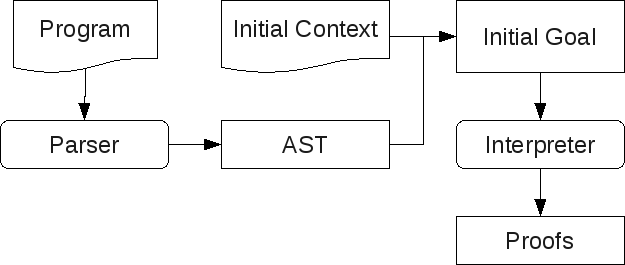
\includegraphics[width=.7\textwidth]{../runtime}
\caption{The \Tcg{} Type Checker at Run Time}
\end{figure}
}

\frame{
	\frametitle{What the interpreter does?}

	$\lambda f : \tau \rightarrow \sigma . \lambda x : \tau . f\,x$

	\begin{tikzpicture}[
		level 1/.style={sibling distance=3cm},
		level 2/.style={sibling distance=1cm}		
		] 
		\node {$\lambda$}
		    child {node {$f$}}
		    child {node {$\rightarrow$}
		    	child {node {$\tau$}}
			child {node {$\sigma$}}
		    }
		    child {node {$\lambda$}
		    	child {node {$x$}}
			child {node {$\tau$}}
			child {node {\texttt{app}}
				child {node {$f$}}
				child {node {$x$}}
			}
		    }
		    ;
                \end{tikzpicture}

}

\frame{
	\frametitle{Components of a \Tcg{} specification}
	A specification in \Tcg{} describes
	\begin{itemize}
		\item Lexicon
		\item Context-Free Syntax
		\item Abstract Syntax
		\item Typing Rules
		\item Pretty-Printing Rules
	\end{itemize}
}

\begin{frame}[fragile]
	\frametitle{Syntax of Simply-Typed $\lambda$-Calculus}
\begin{verbatim}
file: top_wrap EOF {! run ~save: 
                     [ (input.base^".rls",
                       [ ("define", "save_defined") ]) ] 
                     $1 
                   !}
top_wrap: tops        --> tops($1)

tops: top             --> $1 :: []
    | top ";;" tops   --> $1 :: $3

top: exp              --> $1

exp: ID               --> id[$1]
   | exp exp          --> apply($1,$2)
   | "\\" ID "." exp  --> lambda(id[$2],$4)
   | "(" exp ")"      --> $2
\end{verbatim}

\end{frame}

\frame{
	\frametitle{AST production language}
The AST productions are specified after \texttt{'-->'}, the language uses
\begin{itemize}
 \item \code{\$<number>} --- reference items on the left-hand side;
 \item \code{<node_type>(<children>)} --- node constructors;
 \item \code{head::tail} --- lists, \code{[]} is empty list;
 \item \code{<class>[<value>]} --- opaque terms.
\end{itemize}
}

\begin{frame}[fragile]
	\frametitle{Example $\lambda$ expression}
\begin{tabular}{ll}
Mathematical notation: & $(\lambda f.\lambda x. f\; x)\; g\; y$\\
Textual notation: & \code{(\textbackslash f.\textbackslash x.f x) g x}\\
Abstract Syntax Tree:&
\end{tabular}
\begin{center}
	\begin{tikzpicture}[
		level distance=.75cm,
		sibling distance=3cm,
%		level 1/.style={sibling distance=3cm},
%		level 2/.style={sibling distance=1cm}		
		] 
		\node {tops}
		child {node {::}
		    child {node {apply}
		    	child {node {apply}
				child {node {lambda}
					child {node {id[f]}}
					child {node {lambda}
						child {node {id[x]}}
						child {node {apply}
							child {node {id[f]}}
							child {node {id[x]}}
						}
					}
				}
				child {node {id[g]}}
		    	}
			child {node {id[y]}}
		    }
		    child {node {[]}}
		}
		;
                \end{tikzpicture}
\end{center}
%\begin{verbatim}
%tops(
%    apply(
%        apply(
%            lambda(id[f], 
%                lambda(id[x], 
%                    apply(id[f], id[x]))),
%            g),
%        x)
%    ::[]
%)
%\end{verbatim}	
\end{frame}

\begin{frame}[fragile]
	\frametitle{Typing rules}

A conventional typing rule:
\tcgrule{f, e, s, t}{
    \Gamma \vdash f : s \rightarrow t
    \hspace{20pt}
    \Gamma \vdash e : s
}{\Gamma \vdash f\; e : t}{apply}{}

\Tcg{} version:
\begin{columns}
	\column{.5\textwidth}
\begin{verbatim}
rule apply
  forall(f,e,s,t)
    apply(f,e) : t
  if f : fun(s,t)
  and e : s
\end{verbatim}
	\column{.5\textwidth}
\tcgrule{f, e, s, t}{
    \premise{}{f : s \rightarrow t}
    \premise{}{e : s}
}{f\,e : t}{apply}{}
\end{columns}
\end{frame}

\begin{frame}[fragile]
	\frametitle{Context modifiers}
The typing rule in \Tcg{}:
\tcgrule{x, e, s, t}{
    \premise{-( :_1 = x), +[ x : s ]}{e : t}
}{\lambda x. e : fun(s,t)}{lambda}{}
\begin{columns}
	\column{.6\textwidth}
\Tcg{} code:
\begin{verbatim}
rule lambda
  forall(x,e,s,t)
    lambda(x,e) : fun(s,t)
  if e : t
    under -( :.1.= x) + [ x : s ]
\end{verbatim}
	\column{.4\textwidth}
Context modifiers:
\begin{itemize}
	\item \code{-(:.1. = x)} 
	\item \code{+[ x : s ]}
\end{itemize}	
\end{columns}
\end{frame}

\frame{
	\frametitle{The original work}

	Holger Gast, \emph{The Generator for Type Checkers}, University~of~T\"ubingen, 2004

	\footnotesize\url{http://www-pu.informatik.uni-tuebingen.de/users/gast/tcg.html}
}

\end{document}
